\documentclass[11pt]{report}

\usepackage{graphicx}
\usepackage{color} % needed if you use xfig graphics at all
\usepackage{wasysym} 
\usepackage{listings}    
\usepackage{array}
%\usepackage{setspace}

%\doublespacing

\begin{document}
\bibliographystyle{plain}
\newcommand{\plan}[1]{\textcolor{blue}{- \textit{#1}\\}}



\newenvironment{checklist}{%
  \begin{list}{}{}% whatever you want the list to be
  \let\olditem\item
  \renewcommand\item{\olditem -- \marginpar{$\Box$} }
  \newcommand\checkeditem{\olditem -- \marginpar{$\CheckedBox$} }
}{%
  \end{list}
}   

\lstset{language=[Sharp]C}

\title{Web Browser Report\\ Industrial Programming Coursework A}
\author{Duncan Cameron \\
Software Engineering \\
Heriot-Watt University \\
dac31@hw.ac.uk\\
H00153427}
\maketitle

\newpage
\tableofcontents
\chapter{Introduction}

\section{Report Summary}
This report is about the development of the Web Browser application I developed for this coursework task.  The report will detail all of the requirements I met, the considerations I took into account when designing and developing.  It will also include a user and developer guide as well as information on how I tested the program.

\section{Assumptions}
Many of my design decissions were influenced by the book "Clean Code" by Robert C. Martin. The book includes many tips on how to keep code clean from small details such as variable naming to larger ones such as class structure.\\\\
With regards to my assumptions on the specifications I assumed that the multi-threading would be used only for the http requests on each tab, not controlling every aspect of it.  This is as the main form cannot be accessed on any thread other than the one it was created on (which would be the main thread in my programs case).

\chapter{Requirements' Checklist}

As far as I am aware, I managed to implement all requirements from the coursework specification:
\begin{checklist}
	\checkeditem Sending HTTP requests
	\checkeditem Receiving HTTP responses and handling errors
	\checkeditem Home Page
	\checkeditem Favourites, including modification and deletion
	\checkeditem History, including back and forwards buttons
	\checkeditem Tabs
	\checkeditem Multi-threading
	\checkeditem GUI interactions including menu and buttons
	\checkeditem Shortcut keys
\end{checklist}
I also implemented basic html rendering using a library.  However, javascript and css arae not supported the majority of websites look bad in it.  I also implemented navigation by clicking on links on the page.

\chapter{Design Considerations}

\section{Overall Class Design}

The goal of my overall class design was to separate concerns as much as possible, trying enforcing the \textit{Single Responsibility Principal} by giving one responsibility per class.  In practice, this is very hard to do and many of my classes do have more than one, but I still tried to give classes as few responsibilities as possible.  With the form classes this was kind of lost due to the way WinForms work - the class for the form manages all things on the form and handles all of the events  for all the Controls on the form.

Another goal was to try and keep the classes small and readable, with preferably only a few public methods.

\section{The Browser}
The Browser class is central to managing communication and state of the program.  It mainly tracks tabs, what tab is currently active and allows navigation commands to be passed to the tabs.  It also allows the rest of the programs to access the bookmarks and history.

For this class I used a singleton pattern.  The singleton pattern means that only one single instance of the class can ever exist, which is what we want with the Browser class.  It is done by creating a private static variable containing an instance of the class and a public static property to get it.  The constructor is made private so a new one cannot be created anywhere else.  I also had to make sure that it is thread safe, hence the Padlock field and locking it while instantiating the object.

The reason I used a singleton as opposed to a static class is so it can be treated more like an object if need be - it can be assigned to a variable and even passed around as a parameter if need be.

\section{The Main Window}

The MainWindow class handles all events that occur on the GUI.  It also contains a function to set the content that is in the window.

\section{Tabs}

The Tab class controls all that the tabs need to independently function.  It references the tabs LocalHistory to allow for forwards and back navigation.  In order to Load a web page it references the WebHandler class giving it the web page reference and, as a delegate, a function to go to once the html response is retrieved.  This is needed as the request will happen in a new thread and there are different things that will happen depending on how the request was instantiated (e.g. if the link was typed into the browser will act differently than if the back button was pressed.)

\section{Web Handler}

The WebHandler is used to manage http requests and responses.  It also runs the requests on a new thread meaning that the browser can still be used while the request is going on.  It is accessed by one static method, Load Page which creates a new instance of WebHandler and runs it on a new thread.  This means that no other class has to worry about the multi-threaded aspect of the class other than having to pass it a delegate to run once the request is complete.  If there is an error during the process the class will capture it and return that to the delegate instead.  Using the delegate after completion is advantageous as in different situations different things should be done after the completion of the task (e.g. going back will differently effect how history is handled).  It also allows extensibility for further use of requests (e.g. loading CSS files).

\section{Main Panel}

The MainPanel refers to where the content is displayed.  The MainPanelManager class manages the global state of whether the source code or rendered page should be displayed, and alerts all of the panels what one they should show when they are activated - an observer pattern is used here.  This is useful as it alerts the tabs even when they are not active, so when they are activated they know which one to display.

The MainPanels themselves are for the panels for each tab.  They will each have an htmlPanel and a textBox for displaying a rendered page or the source text.  For large web pages, the act of rendering the html can take time and it will cause the whole program to lag as this operation must be done on the main thread.  Therefore it makes sense to only do this if the html mode is active.

This system allows for good performance as pages are not rendered unnecessarily and rendering is faster as the source code is not also displayed "behind the scenes" at the same time.

\section{History, Favourites and Home}

\subsection{Storable Item Hierarchy}

The items that could be stored are made into a certain hierarchy.  

One class notibly used here and throughout the rest of the program is the WebPageReference class.  This class simply contains a field for a url.  While this could just have been a string it is actually useful as it is unable to get confused with other strings and there is no "accidental" functionality that could be incorrectly applied to it.  It also allows extensibility for future functionality e.g. it could be used to verify all urls are valid .  This would require a simple check in the constructor here and not every time a new url is instantiated as a string.

The abstract SavedUrl class contains a WebPageReference and a title.  This is essential for any stored item as we want a title with it too.  It is abstract so its descendants can be easily identified as what they are as no object can be instantiated simply as SavedUrl.  The HistoryItem class inherits from this and adds the time and date when the page was accessed and the HistoryItem was created.  The Bookamrk adds nothing extra but can be easily separated from history items and the like.  The HomePage also inherits from this but adds some extra functionality as it is stored by itself and not as part of a collection.


\subsection{Storable Collection}
The storable collection class was used for global history as well as bookmarks using a generic type T (which was assigned to the Bookmark and HistoryItem class when instantiated in the Browsers constructor).  This class contains simple control functionality for Adding and Removing the items in addition to saving and loading the data.  This is done using the DataStorage class.

\subsection{Data Storage}

To store the History, Favourites and Home page through different executions, they need to be stored.  This is handled by the DataStorage class.  This class uses Generics so it can store and retrieve things of any type (as long as it's Serializable), allowing it to be be used in all 3 cases for the browser.

It uses a binary formatter so the entire object can be stored and then loaded \textit{directly into a new object}.  This method is simple and clean and allows re-usability through generics

\subsection{The Side Panel}

To allow users to access their history and favourites, I create a panel at the side and use that so users can see the favourites or history and display them.  As this takes quite a bit of management, I created the SidePanel class to manage this behaviour.  This detects what state the panel should be in and how it reacts to additional clicks of the favourites or history buttons as well as the job of creating and displaying the buttons in the panel.  I exploited the inheritance structure of the HistoryItem and Bookmark so they can both be run into the same function when creating the buttons.

\subsection{Home}

The way the Home page was stored was slightly different due to not being a collection and having no need for the adding or removing functionality provided in the StorableCollection.  The HomePage class directly inherits form the SavedUrl and deals with data storage internally, by having a DataStorer and adding the public functions SetHomePage and LoadHomePage.  The constructor is also set to private so it cannot be instantiated, only loaded through the LoadHomePage function that uses the DataStorer or CreateHomePage (which also uses the DataStorer that has already been instantiated) to set the initial one if loading failed.

\section{Other Remarks}

Another goal to keep my code clean and understandable was through the use of naming and comments.  I would rely mainly on variable, function and class names and only use comments when necessary (as is advised in "Clean Code").  I also aimed to keep functions short and not contain too many indentations so any programmer looking at the code can easily see what is happening.  This also reduces the need for comments as the function name can clearly describe what the section of code is about.

\chapter{User Guide}

This is the user guide which details how to use the features in the browser.  Screenshots can be found in the appendix

\section{Loading A WebPage}

To load a web page, enter a url in the text bar at the top of the window and either click "Go" or press return on the keyboard.

\section{Navigating Back and Forwards}

Clicking the button "\textless-" will navigate back a page and "-\textgreater" will navigate forwards a page.

\section{Saving Favourites}

To save an item to your favourites click the "Add to favourites" button.

\section{Accessing Favourites and History}

Pressing the "Favourites" or "History" button will bring up the favourites or history on the right side of the screen.  Click one of the buttons to navigate to the page it references.  History items can be deleted here, or favourites can be edited.

\section{Setting The Home Page}

To set the homepage, navigate to the page you want as your home using the url bar and, under the options menu, press "Set current page as home".

\section{Tabs}

Pressing the "+" icon will open a new tab.  Clicking on different tabs along the tab bar will change which one is displayed.  Clicking the "X" next to a tab will close it.  Within tabs new pages can be opened simultaneously, and navigation for forwards and back is stored independently for each tab.

\section{Viewing The Source Code}

To view the source code press the "View Source" button.  To return to rendered html, press the "Show Rendered Page" button.

\section{Keyboard Shortcuts}

There are several shortcut keys implemented into the browser in order to speed up use:
\begin{itemize}
\item ALT left - back
\item ALR right - forwards
\item F5 - refresh
\item CTRL H - open history
\item CTRL B - open favourites
\item CTRL T - open new tab
\end{itemize}

\chapter{Developer Guide}

\section{The Browser}

The main browser class allows access to many aspects of the browser, including the tabs, history and bookmarks.  It uses a singleton pattern and can be accessed globally through calling:
\begin{lstlisting}
Browser.Instance
\end{lstlisting}

\section{Tabs}

The Tab class contain methods to navigate through different web pages.  In the fields they keep track of data concerning the currently loaded page (such as a reference to the page containing the url, the html content of the page and whether the forwards and back buttons should be active.

When a tab is created, it also creates a new button and puts it onto the main form (along with a close button) so the user can switch between different tabs.  There are also various methods to load a new web page under different circumstances (e.g. from the url bar, back, forwards, refresh), as well as functions for what to do what a page has been loaded under different circumstances.

When the form is to be updated with the latest page, it must be done in an invoke statement.  This is as the delegates for when a web response is received is in a different thread and it will not be able to update the form.

\section{Web Requests}

The WebHandler class will create a web request and get the response.  The response is then sent to whatever delegate was passed into the WebRequest on creation.  To make a request, the static "LoadPage" function should be used - it will deal with instantiation and multi-threading.  If an error occurred, the message will be passed instead of the content. Here is an example on how to make a request:

\begin{lstlisting}
public void StartLoadingWebPage(WebPageReference webPage) {
	WebHandler.LoadPage(webPage, DealWithReponse);
	Console.WriteLine("The request has been sent");
	DoSomeOtherStuffWhileThePageIsLoading()
}

private void DealWithResponse(string content, WebPageReference webPage) {
	Console.WriteLine("The web page response has arrived!");
	Console.WriteLine(content);
}
\end{lstlisting}

\section{Data Storage}

The DataStorer class deals with storing the data for Bookmarks, History and Home Page.  When one is created it needs a file location and then data can be saved or loaded from there.  It reatians the form of whatever type the Generic Type used to create it with was.  It uses a BinaryFormatter to serialize the data, so any object that is to be stored must be of a serializable type.

The StorableCollection is used to store a list of things with functionality to easily add, remove and save - it also makes sure that it is saved whenever it is updated.

\section{Side Panel}

The SidePanel class manages the side panel on the main form for accessing the history and bookmarks.  It manages which one should be active and sets it up for the appropriate usage.  This includes setting up the buttons in the panel as well.

\section{Main Panel}

The MainPanel controls the state for each tab on the form, between being a rendered page or displaying the source code.  The MainPanelManager controls the global state and will update all the panels when the mode is changed - an observer pattern is being used here.

The MainPanel will then only display on the correct output to ensure stronger performance.  Note that setting the text to the sourcebox or htmlPanel can be slow and lag the whole system as it must be done on the main thread.

\section{Main Window}

The main window controls all of the events that occur when a user interacts with the window.  It also handles the shortcuts from key inputs.  In the constructor it will set-up some aspects for the window to display properly.

\chapter{Testing}

To ensure that the program would correctly function under all conditions, the program was tested by trying to perform all possible actions and make sure that program behaves as expected.  Testing was done continuously throughout the development by testing debug builds and trying to make errors occur.  I also inserted Code Contracts at various places in my code to ensure that the program was behaving correctly.

Through testing I found no way to crash the program, but did come across a few issues that could be corrected:\\
\begin{itemize}
\item If "Add To Favourites" is pressed while the favourites side panel is up, it will not be updated and the item will not appear until the panel has been closed and reopened - the same thing happens if a new page is loaded while the history panel is open.
\item Some websites will not correctly have their titles set - this results in incorrect tab headings and entries into history and favourites.  This is because I use a regex to find the title but there are cases where the regex does not work as it looks for a field exactly matching "$<$title$>$" - this will ignore cases such as "$<$title id='titleid3'$>$" or similar.
\item Tabs can keep being opened infinitely even when there is no way to access them as they have been pushed of the edge of the screen.  A way to fix this could be to implement a hard number of tabs that can remain open or to set the panel to have a scroll bar so all opened tabs can be accessed
\item When showing the history when there is a lot of items there it causes the program to lag as many buttons are being added.  It would perhaps be better to display it as text or using some less resource heavy way of displaying the information.
\end{itemize}

\chapter{Conclusion}

I believe that my browser was well designed and utilised many features of c\# in order to do so.

One part that I am proud of was my WebHandler class - it managed to create a thread, instantiate an instance of the class, make a web request, receive a response and handle errors all in 52 lines of code (many of which were comments or blank).  It was also easy and simple to use and meant that other parts of the code did not have to worry too much about multi-threading (some methods still had to return to the main thread to update the form).

I also think that my overall design was fairly simple and effective at appropriately separating responsibilities across different classes.

One thing that I think could be improved upon a lot is the user interface.  It is fairly ugly through the use of a lot of buttons and often clunky to use.   I would also have liked to make the url bar expand across the available screen but I was unable to figure out how to do this using the Winforms GUI system

\chapter{Appendix}
\section{Screenshots}
\subsection{Main Browser}
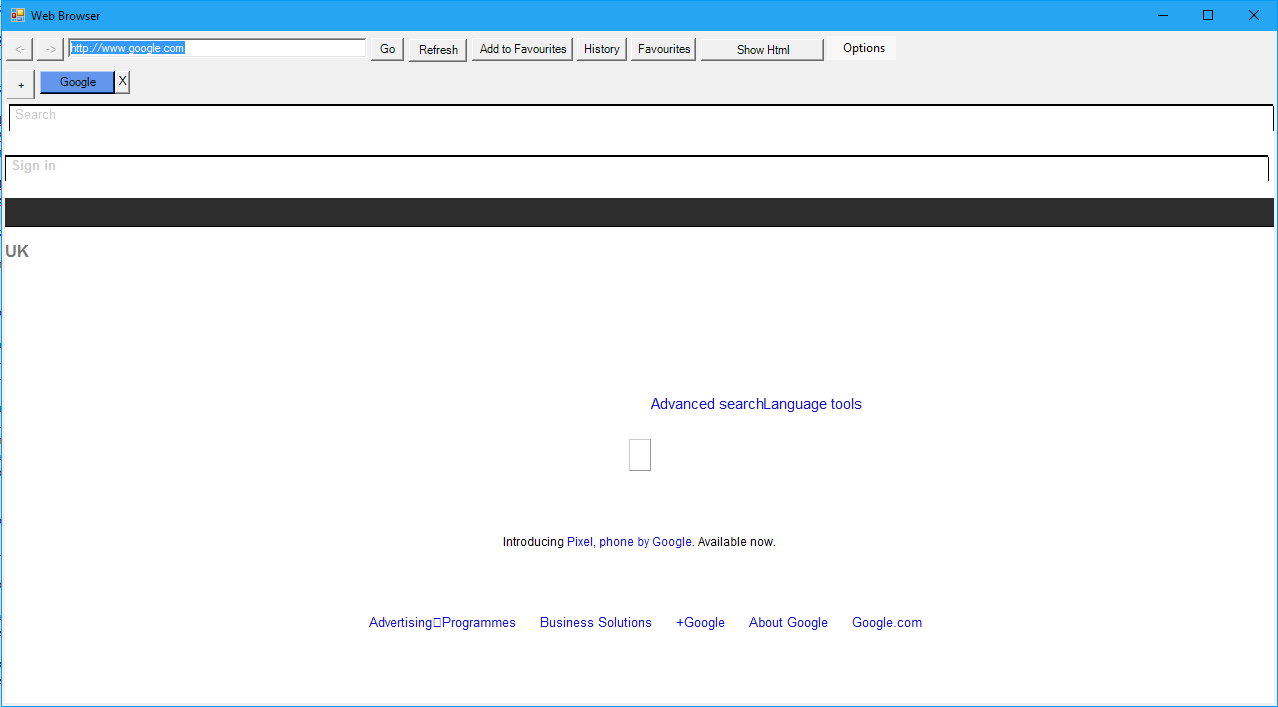
\includegraphics[scale=0.4]{browser.png}
\subsection{History Panel}
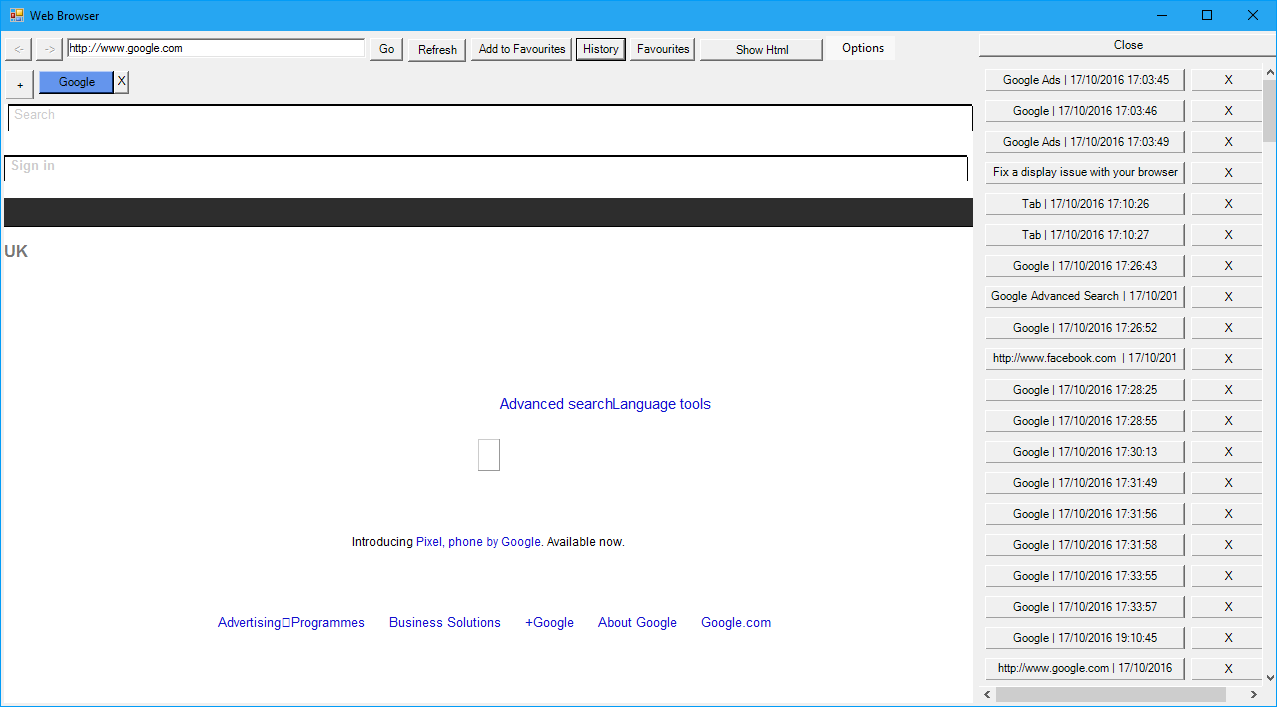
\includegraphics[scale=0.4]{history.png}
\subsection{Favourites Panel}
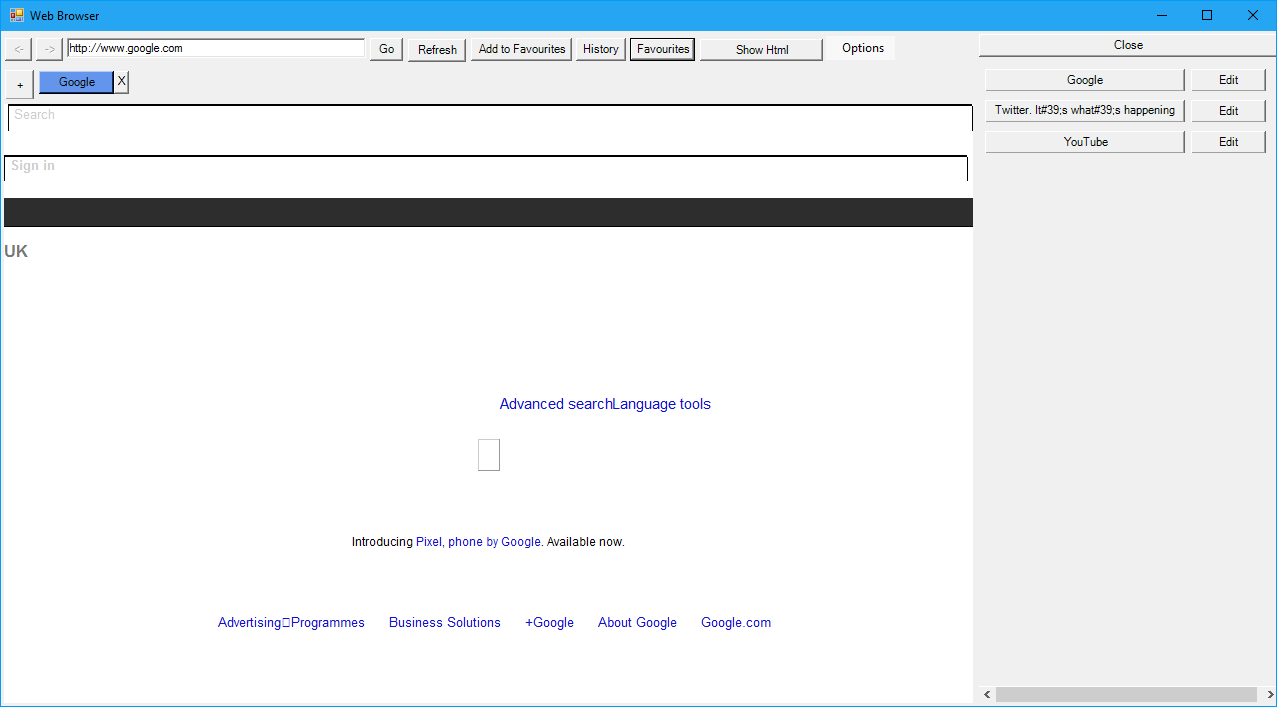
\includegraphics[scale=0.4]{favourites.png}
\subsection{Editing Favourites}
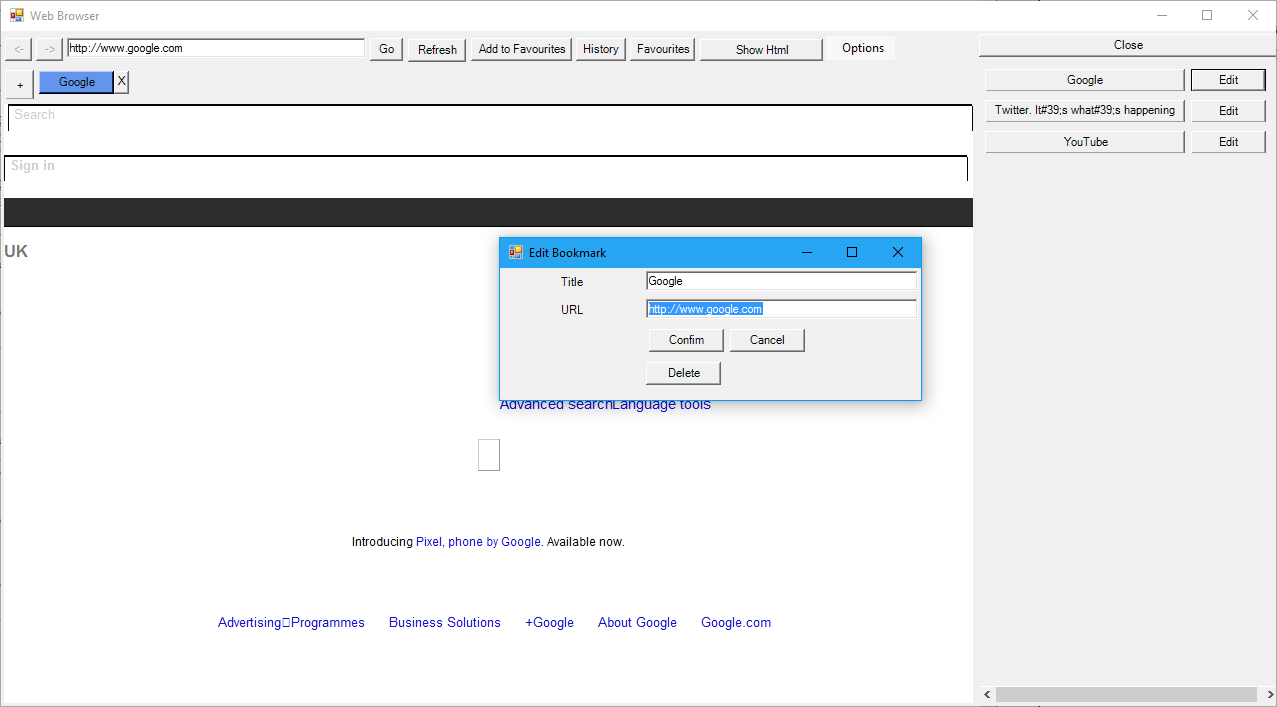
\includegraphics[scale=0.4]{edit-favourites.png}
\subsection{Showing Source}
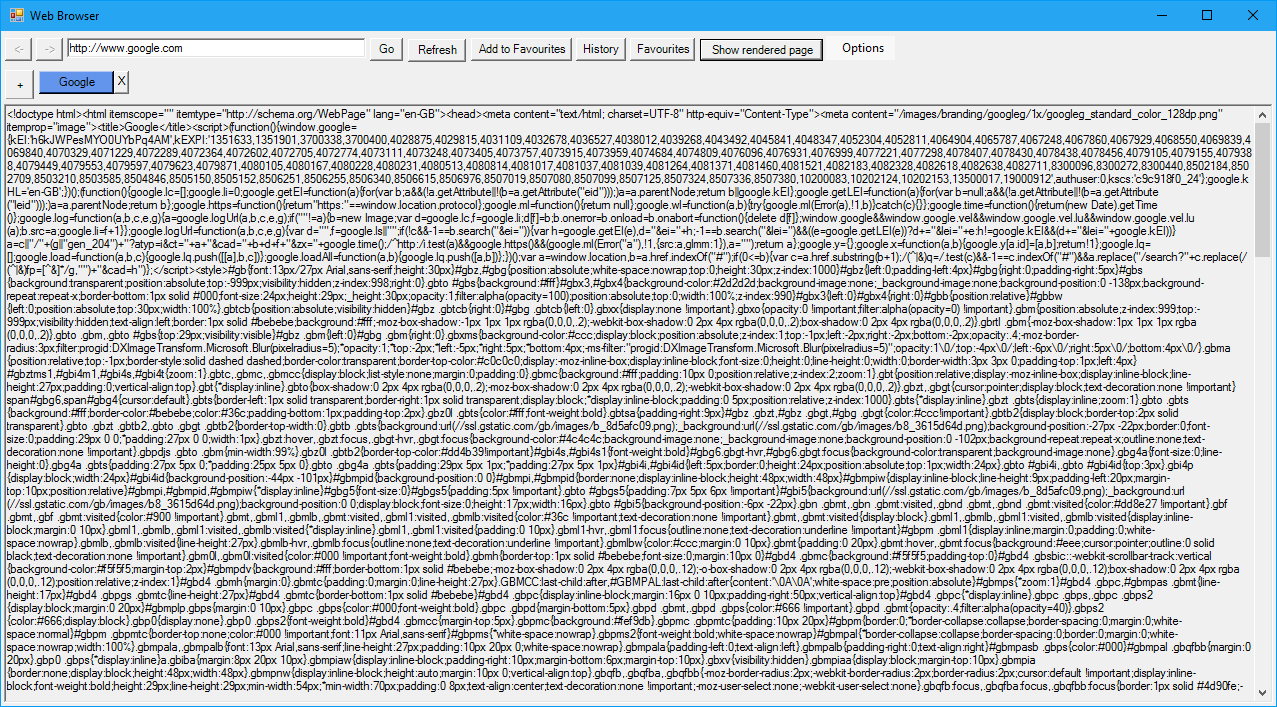
\includegraphics[scale=0.4]{source.png}
\subsection{Options}
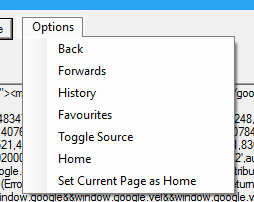
\includegraphics[scale=1]{options.png}


\end{document}